\chapter{Návrh řešení}
Tato kapitola se věnuje návrhu webové aplikace, která přímo vychází z teoretických poznatků o reaktivních systémech a z analýzy požadavků definovaných v kapitole \ref{sec:analyza_pozadavku}. 
Cílem tohoto návrhu je vytvořit modulární a uživatelsky přívětivé prostředí, které studentům i vyučujícím usnadní práci s formálními modely. 
Architektura je koncipována tak, aby oddělovala prezentační logiku od výpočetního jádra, což umožňuje flexibilní rozšiřování aplikace. 
Návrh konkrétní implementace a detailní popis použitých algoritmů jsou následně předmětem kapitoly \ref{sec:implementace}.

\section{Případy užití}

Pro správné navržení uživatelského rozhraní a aplikační logiky je nezbytné definovat, jakým způsobem budou uživatelé s aplikací interagovat. 
Systém je navržen tak, aby spolehlivě obsloužil několik základních scénářů pokrývajících potřeby studentů i pedagogů. 

Mezi hlavní případy užití ze strany uživatele jako studenta patří:
\begin{itemize}
    \item \textbf{Samostatné procvičování látky:} 
    Student si může ověřit a upevnit své znalosti z oblasti formální verifikace. 
    Po spuštění aplikace má k dispozici sadu předpřipravených příkladů, dostupné na jedno kliknutí. 
    Na těchto příkladech má možnost krokovat odvozování syntaxe, vizualizovat grafy nebo interaktivně dokazovat přechody pomocí pravidel strukturální operační sémantiky.
    \item \textbf{Řešení zadaných úkolů:} 
    Student obdrží od vyučujícího konkrétní příklady (například ve formě exportovaného \texttt{.json} souboru), které snadno naimportuje do svého pracovního prostředí. 
    V něm danou problematiku analyzuje, příklad vyřeší a následným exportem odevzdá vyučujícímu.
    \item \textbf{Tvorba vlastních příkladů:} 
    Uživatel může v aplikaci založit zcela nový projekt, ve kterém si nadefinuje vlastní procesy kalkulu komunikujících systémů, odpovídající LTS grafy či důkazy přechodů. 
    Tato funkcionalita je využitelná například při řešení zápočtových projektů nebo pokud si chce student sám něco zkusit vytvořit k procvičení.
\end{itemize}

Případy užití z pohledu vyučujícího zahrnují:
\begin{itemize}
    \item \textbf{Plný rozsah studentských případů užití.}
    \item \textbf{Interaktivní ukázky ve výuce:} 
    Vyučující může aplikaci aktivně prezentovat během přednášek či cvičení. 
    Namísto vypisování důkazů na tabuli lze v aplikaci demonstrovat přechod mezi stavy krok za krokem, striktně podle formálních pravidel SOS. 
    Tento přístup může výuku zrychlit a studenty motivovat, aby si předváděné postupy následně zkusili dokázat sami.
    \item \textbf{Příprava výukových materiálů:} 
    Pedagog může v aplikaci navrhnout specifické modely LTS, které vizualizují nejrůznější stavy a přechody. 
    Tyto modely lze následně exportovat ve formě obrázků nebo datových souborů, které se mohou dále využít například při tvorbě prezentací. 
    Stejným způsobem byly vytvořeny obrázky \ref{fig:ccs_parallel} a \ref{fig:ccs_sync_restricted} z kapitoly \ref{sec:reaktivni_systemy}.
\end{itemize}

Po spuštění aplikace má uživatel rychlý přístup k nápovědě umístěné v pravé části hlavičky stránky, která objasňuje základní principy ovládání a fungování aplikace.
Tuto nápovědu i celý program si také může přeložit tlačítkem volby jazyka, která se nachází vedle nápovědy. 
V hlavním rozcestníku si uživatel volí, zda chce pracovat s předdefinovaným programem, importovat existující, nebo vytvořit program zcela nový. 
Všechny tyto případy užití jsou ve zjednodušené podobě znázorněny na obrázku \ref{fig:use_case}.

\begin{figure}[h!]
    \centering
    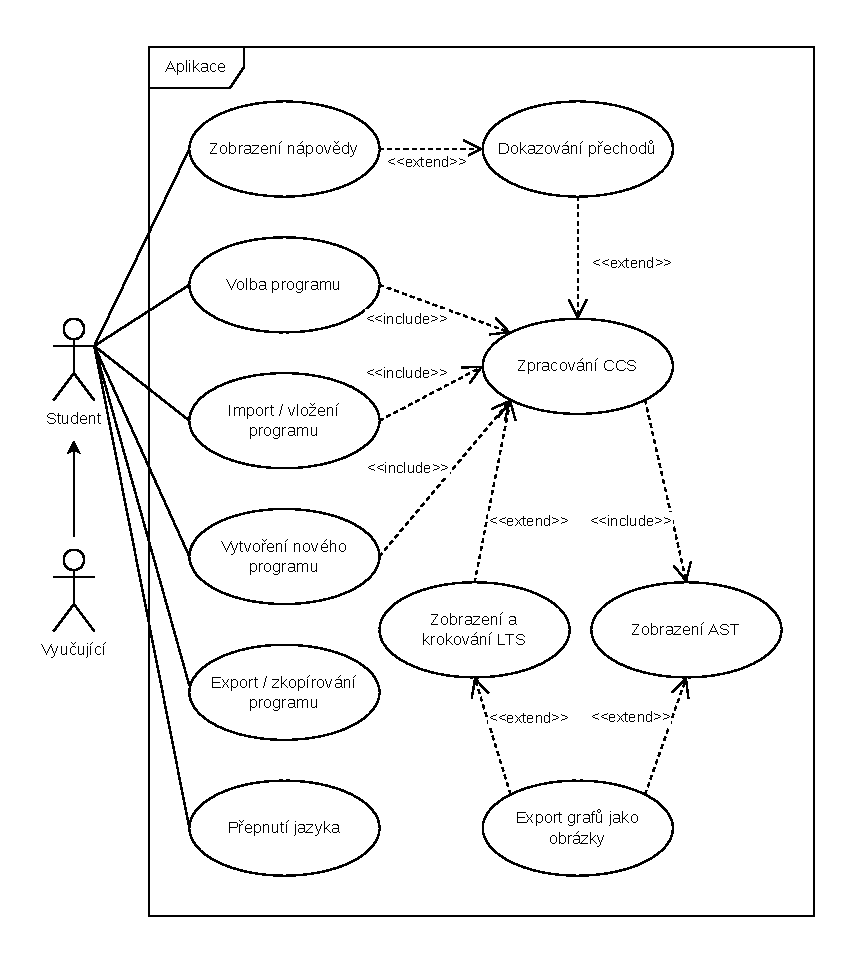
\includegraphics[width=0.93\textwidth]{Figures/usecase.pdf}
    \caption{UML diagram hlavních případů užití aplikace}
    \label{fig:use_case}
\end{figure}

\section{Návrh datových struktur}

Pro efektivní abstrakci jednotlivých komponent aplikace bylo nutné navrhnout datové toky a vnitřní reprezentaci uživatelských vstupů. 
Z uživatelského hlediska aplikace přijímá jako vstup textovou definici CCS procesů. 
Tento vstup je v první fázi zpracován syntaktickým analyzátorem, který vstupní text transformuje do abstraktního syntaktického stromu ve formátu JSON. 

Nad tímto stromem jsou posléze vystavěny další datové struktury nezbytné pro vnitřní logiku aplikace. 
Jedná se především o struktury pro generování vrcholů a hran grafu LTS, syntaktického stromu a struktury pro dokazování přechodů pomocí SOS pravidel. 
Detailní popis těchto struktur a procesu parsování je podrobněji rozebrán v kapitole \ref{sec:struct_format}.

\section{Architektura webové aplikace}

Aplikace je navržena jako Single-Page Application (SPA) s využitím knihovny React.js. 
Celý návrh dodržuje princip oddělení zodpovědností (Separation of Concerns). 
Zdrojové kódy a aplikační logika jsou logicky rozděleny do dvou hlavních vrstev, reprezentovaných adresářovou strukturou projektu:
\begin{itemize}
    \item \textbf{Vrstva aplikační logiky (adresář \texttt{lib}):} 
    Zajišťuje zapouzdření doménové logiky celého systému. 
    Obsahuje pouze funkce, které nejsou závislé na uživatelském rozhraní. 
    Nachází se zde například zpracování uživatelského vstupu, generátor syntaktického stromu či algoritmy pro výpočet stavových prostorů i přechodů pro LTS, včetně přípravy struktury pro následné vykreslení grafu.
    \item \textbf{Vrstva uživatelského rozhraní (adresář \texttt{components}):} 
    Vrstva sdružuje veškeré vizuální a interaktivní prvky aplikace, navržené jako znovupoužitelné komponenty.
    Součástí této vrstvy jsou také UI prvky z knihovny \texttt{shadcn/ui}, které tak mohou být funkčně přizpůsobeny potřebám projektu.
\end{itemize}

Základní adresář komponent je dále hierarchicky členěn podle své funkčnosti, viz obrázek \ref{fig:component_structure}. 
Mezi základní funkční celky patří \texttt{TextEditor}, obalující knihovnu CodeMirror pro zápis CCS a syntakticky strom, \texttt{SOSProofer} pro vše potřebné z oblasti interaktivní konstrukce důkazů a \texttt{LTSGraph} pro všechny komponenty specifické pro zobrazení LTS grafu. 
Klíčovou roli hraje \texttt{ProgramsContext}, který centralizovaně spravuje stavy aplikace jakožto jediný zdroj pravdy (Single Source of Truth). Tímto přístupem se zamezuje desynchronizaci dat napříč komponentami.
Veškeré úkony spojené s globální správou programů, jako je jejich vytváření, aktualizace, mazání a obecně práce s dynamicky generovanými kartami, jsou zpracovávany komponentami z \texttt{ProgramsSelector}.

\begin{figure}[h!]
    \centering
    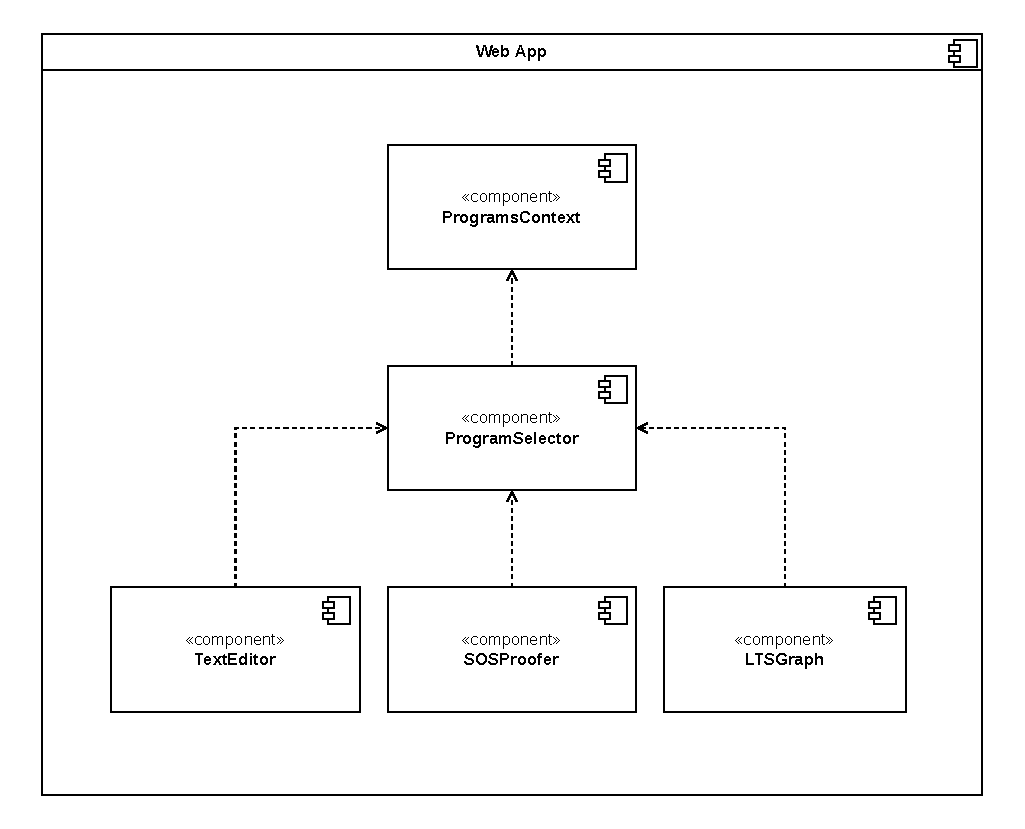
\includegraphics[width=0.95\textwidth]{Figures/components.pdf}
    \caption{UML diagram architektury aplikace}
    \label{fig:component_structure}
\end{figure}

\section{Uživatelské rozhraní}

Návrh uživatelského rozhraní klade důraz na interaktivitu, plynulost a přehlednost. 
Uživatelské prostředí se skládá z jediné dynamické stránky, jejíž obsah je spravován prostřednictvím překryvných modálních oken a variabilního systému karet, zobrazených na obrázku \ref{fig:card_ui}.

\begin{figure}[h!]
    \centering
    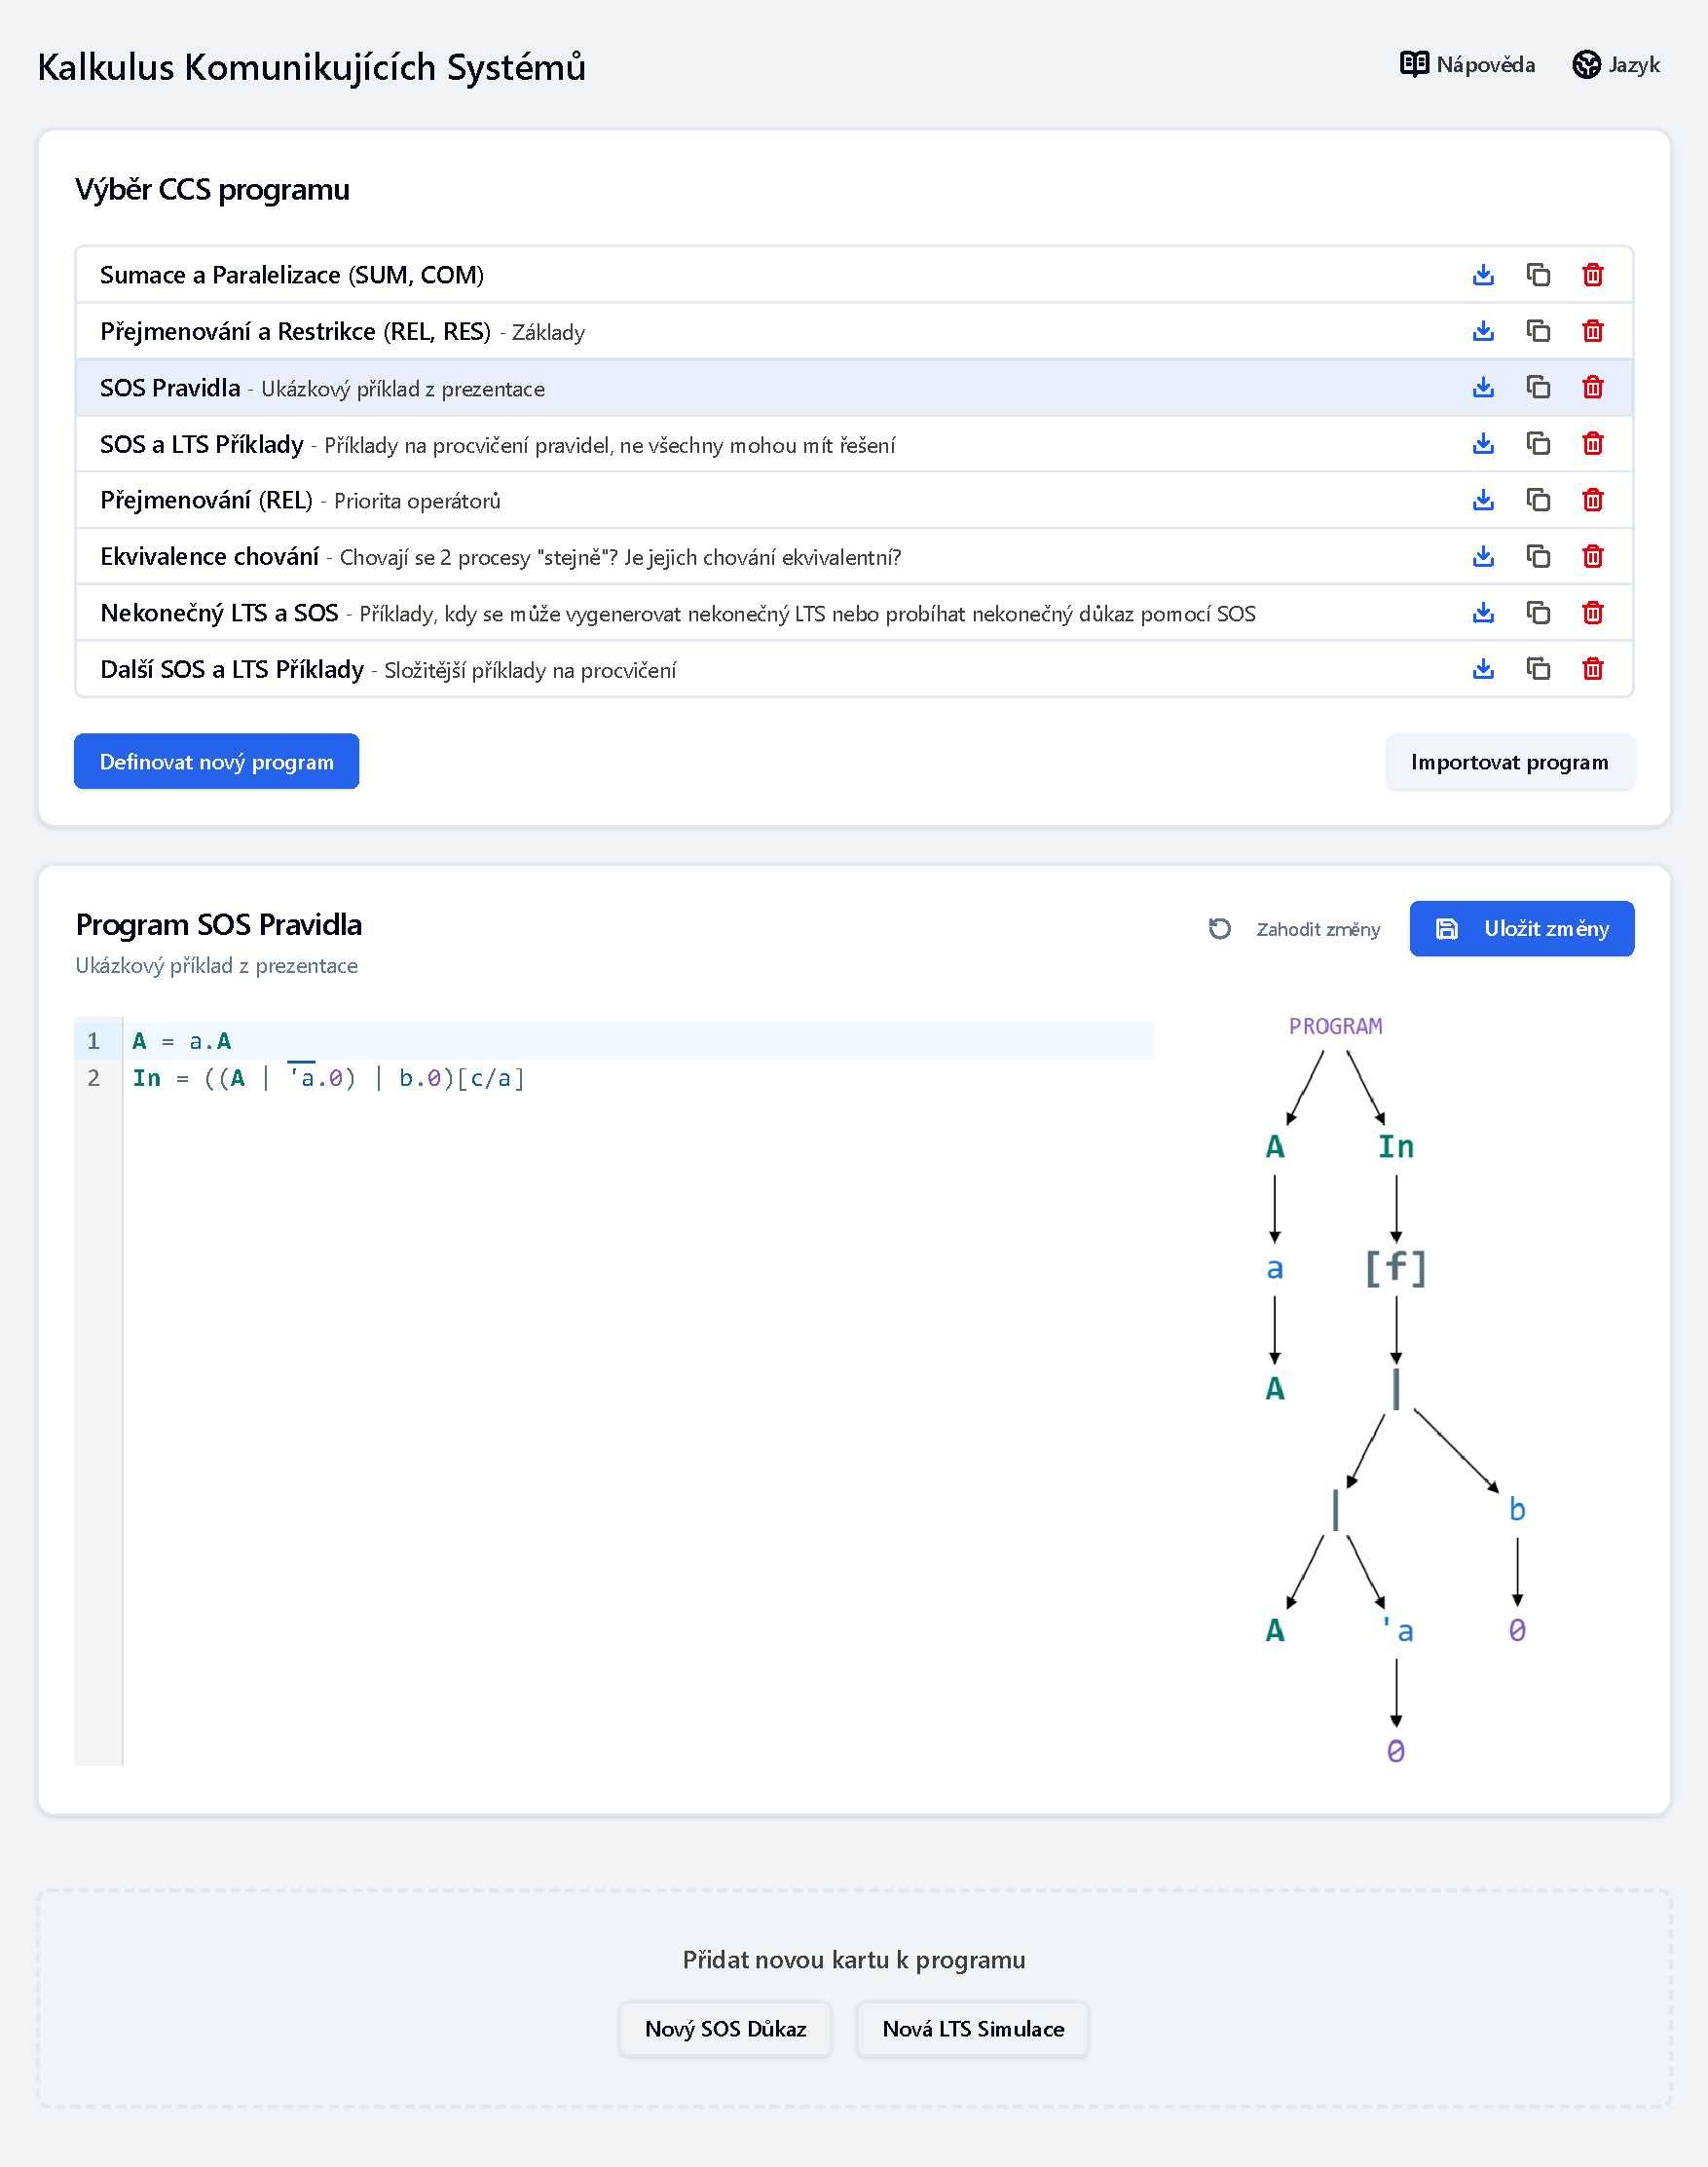
\includegraphics[width=0.98\textwidth]{Figures/card_ui.pdf}
    \caption{Uživatelské rozhraní založené na systému karet}
    \label{fig:card_ui}
\end{figure}

Při úvodním načtení aplikace vidí uživatel pouze výchozí kartu určenou k výběru programu. 
Zde má uživatel možnost načíst již vytvořený program, importovat vlastní zadání, nebo přes dialogové okno vytvořit program zcela nový. 
Hlavička stránky zůstává neměnná a nabízí změnu lokalizace i vyvolání nápovědy.

Jakmile je program zvolen či vytvořen, systém dynamicky vygeneruje hierarchicky podřazené karty. 
Výchozím a trvale přítomným prvkem je karta textového editoru. 
Uživatel v ní zadává definice procesů CCS, přičemž editor v reálném čase provádí validaci vstupu a graficky upozorňuje na případné syntaktické chyby. 
Při úspěšné validaci výrazu se ve stejné kartě rovněž automaticky vykresluje struktura syntaktického stromu.
Kromě textového editoru může k jednomu programu náležet libovolné množství dalších podkaret. Ty mohou být dvou typů:
\begin{enumerate}
    \item \textbf{Karta důkazu SOS:} 
    Nabízí interaktivní prostředí pro krokovou konstrukci důkazu přechodu z jednoho CCS výrazu do druhého za využití formálních pravidel strukturální operační sémantiky.
    \item \textbf{Karta LTS:} 
    Zajišťuje vizualizaci ohodnocených přechodových systémů, kde jednotlivé vrcholy grafu reprezentují dosažitelné stavy programu a hrany odpovídají akcím, které mění jeho stav.
\end{enumerate}

Na konci zobrazení podkaret je umístěna silueta karty, fungující jako rozcestník pro přidávání dalších karet obou zmíněných typů. 
Aby si uživatel udržel orientaci při vysokém počtu karet, umožňuje rozhraní každou z nich individuálně pojmenovat (funkcí editace v pravém horním rohu karty) a popsat tak, jakou konkrétní část systému daná karta vizualizuje či dokazuje. 
U vybraných karet je také dostupná nápověda pro specifické funkce karty. 
V případě, že je program explicitně uzamčen proti úpravám, přejde uživatelské rozhraní do režimu pouze pro čtení, kde není možné měnit obsah editoru a nelze jakkoli manipulovat s kartami.

\endinput